%%%%%%%%%%%%%%%%%%%%%%%%%%%%%%%%%%%%%%%%%
% Beamer Presentation
% LaTeX Template
% Version 1.0 (10/11/12)
%
% This template has been downloaded from:
% http://www.LaTeXTemplates.com
%
% License:
% CC BY-NC-SA 3.0 (http://creativecommons.org/licenses/by-nc-sa/3.0/)
%
%%%%%%%%%%%%%%%%%%%%%%%%%%%%%%%%%%%%%%%%%

%----------------------------------------------------------------------------------------
%	PACKAGES AND THEMES
%----------------------------------------------------------------------------------------

\documentclass[UTF8,aspectratio=169,14pt]{ctexbeamer}

\usepackage{hyperref}
\hypersetup{
	colorlinks=true,
	linkcolor=red,
	anchorcolor=blue,
	citecolor=green
}

\mode<presentation> {
	
	% The Beamer class comes with a number of default slide themes
	% which change the colors and layouts of slides. Below this is a list
	% of all the themes, uncomment each in turn to see what they look like.
	
	%\usetheme{default}
	%\usetheme{AnnArbor}
	%\usetheme{Antibes}
	%\usetheme{Bergen}
	%\usetheme{Berkeley}
	%\usetheme{Berlin}
	%\usetheme{Boadilla}
	%\usetheme{CambridgeUS}
	%\usetheme{Copenhagen}
	%\usetheme{Darmstadt}
	%\usetheme{Dresden}
	%\usetheme{Frankfurt}
	%\usetheme{Goettingen}
	%\usetheme{Hannover}
	%\usetheme{Ilmenau}
	%\usetheme{JuanLesPins}
	%\usetheme{Luebeck}
	\usetheme{Madrid}
	%\usetheme{Malmoe}
	%\usetheme{Marburg}
	%\usetheme{Montpellier}
	%\usetheme{PaloAlto}
	%\usetheme{Pittsburgh}
	%\usetheme{Rochester}
	%\usetheme{Singapore}
	%\usetheme{Szeged}
	%\usetheme{Warsaw}
	
	% As well as themes, the Beamer class has a number of color themes
	% for any slide theme. Uncomment each of these in turn to see how it
	% changes the colors of your current slide theme.
	
	%\usecolortheme{albatross}
	%\usecolortheme{beaver}
	%\usecolortheme{beetle}
	%\usecolortheme{crane}
	%\usecolortheme{dolphin}
	%\usecolortheme{dove}
	%\usecolortheme{fly}
	%\usecolortheme{lily}
	%\usecolortheme{orchid}
	%\usecolortheme{rose}
	%\usecolortheme{seagull}
	%\usecolortheme{seahorse}
	%\usecolortheme{whale}
	%\usecolortheme{wolverine}
	
	%\setbeamertemplate{footline} % To remove the footer line in all slides uncomment this line
	%\setbeamertemplate{footline}[page number] % To replace the footer line in all slides with a simple slide count uncomment this line
	
	%\setbeamertemplate{navigation symbols}{} % To remove the navigation symbols from the bottom of all slides uncomment this line
}

\usepackage{graphicx} % Allows including images
\graphicspath{{./figs/}}
\usepackage{booktabs} % Allows the use of \toprule, \midrule and \bottomrule in tables
\usepackage{longtable}
\usepackage{listings}
\usepackage{xcolor}
\lstset{numbers=left, %设置行号位置
	numberstyle=\tiny, %设置行号大小
	keywordstyle=\color{blue}, %设置关键字颜色
	commentstyle=\color[cmyk]{1,0,1,0}, %设置注释颜色
	frame=single, %设置边框格式
	escapeinside=``, %逃逸字符(1左面的键),用于显示中文
	%breaklines, %自动折行
	extendedchars=false, %解决代码跨页时,章节标题,页眉等汉字不显示的问题
	xleftmargin=2em,xrightmargin=2em, aboveskip=1em, %设置边距
	tabsize=4, %设置tab空格数
	showspaces=false %不显示空格
}
% Fonts
% \usepackage{libertine}
% \setmonofont{Courier}
\setCJKsansfont[ItalicFont=Noto Serif CJK SC Black, BoldFont=Noto Sans CJK SC Black]{Noto Sans CJK SC}


%----------------------------------------------------------------------------------------
%   TITLE PAGE
%----------------------------------------------------------------------------------------

\title[第4讲]{第四讲 物理内存管理 :连续内存分配} % The short title appears at the bottom of every slide, the full title is only on the title page
\subtitle{第2节 再看程序的地址空间}
\author{向勇、陈渝} % Your name
\institute[清华大学] % Your institution as it will appear on the bottom of every slide, may be shorthand to save space
{
清华大学计算机系 \\ % Your institution for the title page
\medskip
\textit{xyong,yuchen@tsinghua.edu.cn} % Your email address
}
\date{\today} % Date, can be changed to a custom date

\begin{document}

\begin{frame}
\titlepage % Print the title page as the first slide
\end{frame}

%----------------------------------------------------------------------------------------
%\begin{frame}
%\frametitle{提纲} % Table of contents slide, comment this block out to remove it
%\tableofcontents % Throughout your presentation, if you choose to use \section{} and \subsection{} commands, these will automatically be printed on this slide as an overview of your presentation
%\end{frame}

%----------------------------------------------------------------------------------------
%   PRESENTATION SLIDES
%----------------------------------------------------------------------------------------
%------------------------------------------------
\section{第2节 再看程序的地址空间}% Sections can be created in order to organize your presentation into discrete blocks, all sections and subsections are automatically printed in the table of contents as an overview of the talk
%------------------------------------------------
\subsection{地址空间} % A subsection can be created just before a set of slides with a common theme to further break down your presentation into chunks
%------------------------------------------------
\begin{frame}[plain,t]
    \frametitle{地址空间定义}
    \begin{columns}
        \begin{column}{0.5\textwidth}
		    \begin{figure}
		        \centering
		%        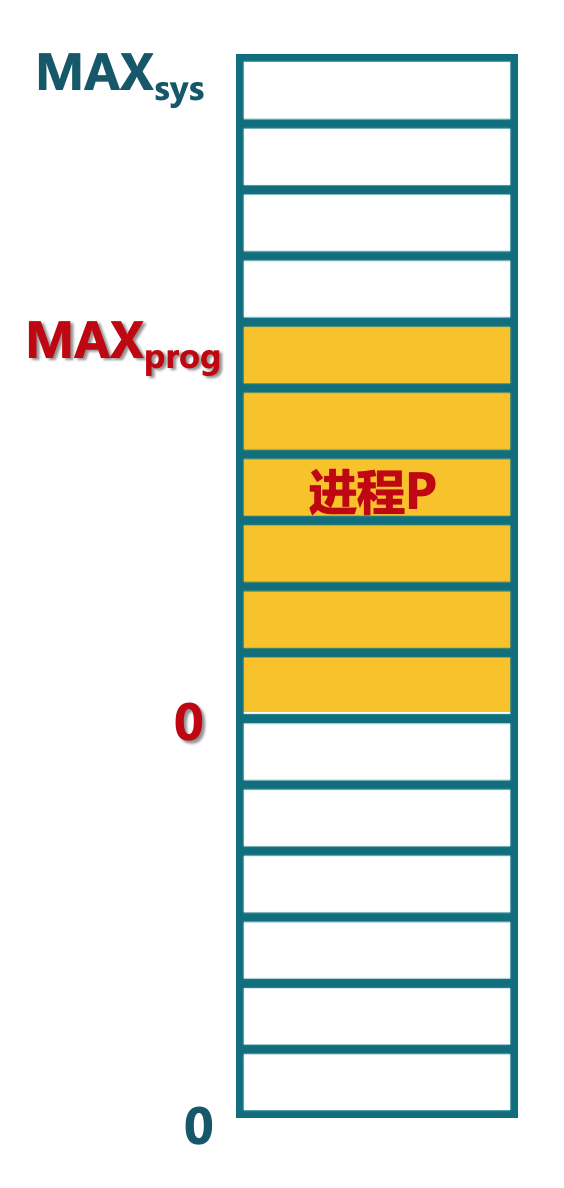
\includegraphics[width=0.7\linewidth]{address-space}
		%        \caption{xxxx}
		    \end{figure}
        \end{column}
        \begin{column}{0.5\textwidth}
			\begin{itemize}
			    \item 物理地址空间 — 硬件支持的地址空间
			    \begin{itemize}
				    \item 起始地址0,直到\begin{math}MAX_{sys}\end{math}
			    \end{itemize}
			    \item 逻辑地址空间 — 在CPU运行的进程看到的地址
			    \begin{itemize}
			        \item 起始地址0,直到\begin{math}MAX_{prog}\end{math}
			    \end{itemize}
			\end{itemize}
        \end{column}
    \end{columns}
\end{frame}
%------------------------------------------------

\subsection{地址生成} % A subsection can be created just before a set of slides with a common theme to further break down your presentation into chunks
%------------------------------------------------

\begin{frame}[plain,t]
    
    \frametitle{逻辑地址生成}
    \begin{figure}
        \centering
%        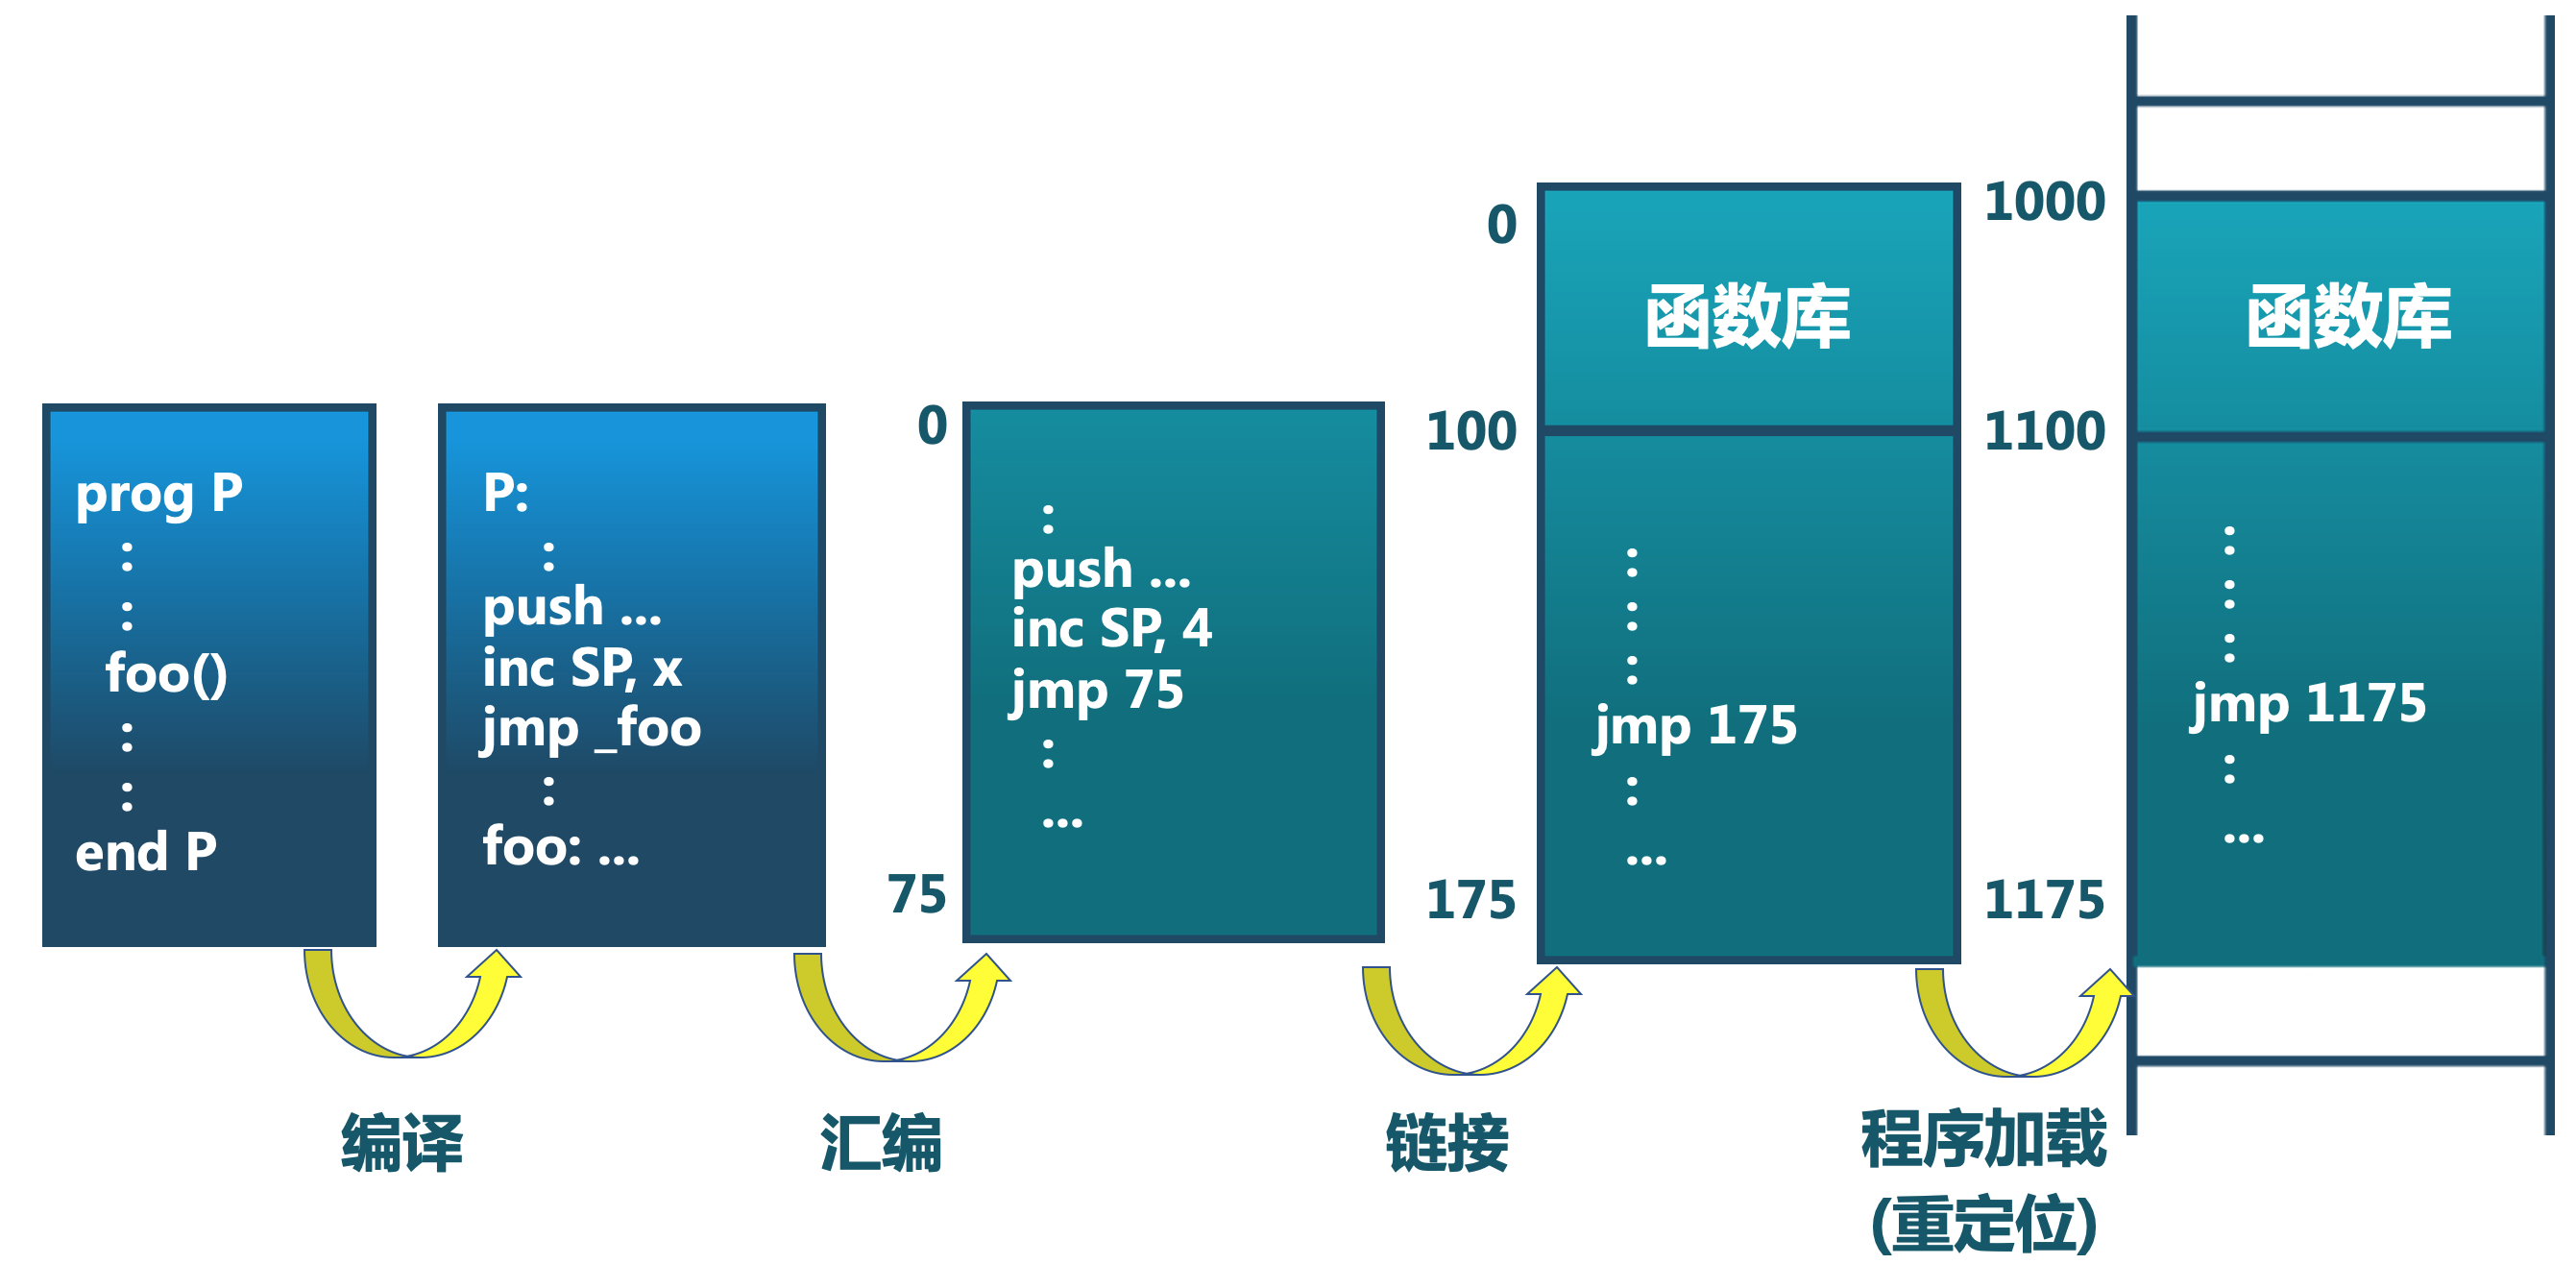
\includegraphics[width=0.7\linewidth]{add-generation}
%        \caption{xxxx}
    \end{figure}
    
\end{frame}
%------------------------------------------------
\begin{frame}[plain,t]
    \frametitle{地址生成时机和限制}
	\begin{itemize}
	    \item 编译时
	    \begin{itemize}
	        \item 假设起始地址已知
	        \item 如果起始地址改变,必须重新编译
	    \end{itemize}
	    \item 加载时
	    \begin{itemize}
	        \item 如编译时起始位置未知,编译器需生成可重定位的代码(relocatable code) 
	        \item 加载时,生成绝对地址
	    \end{itemize}
	    \item 执行时
	    \begin{itemize}
	        \item 执行时代码可移动
	        \item 需地址转换(映射)硬件支持
	    \end{itemize}
	\end{itemize}    
\end{frame}
%------------------------------------------------
\begin{frame}[plain,t]
    
    \frametitle{地址生成过程}
    
	\begin{columns}
	    \begin{column}{0.5\textwidth}
		    \begin{figure}
		        \centering
		        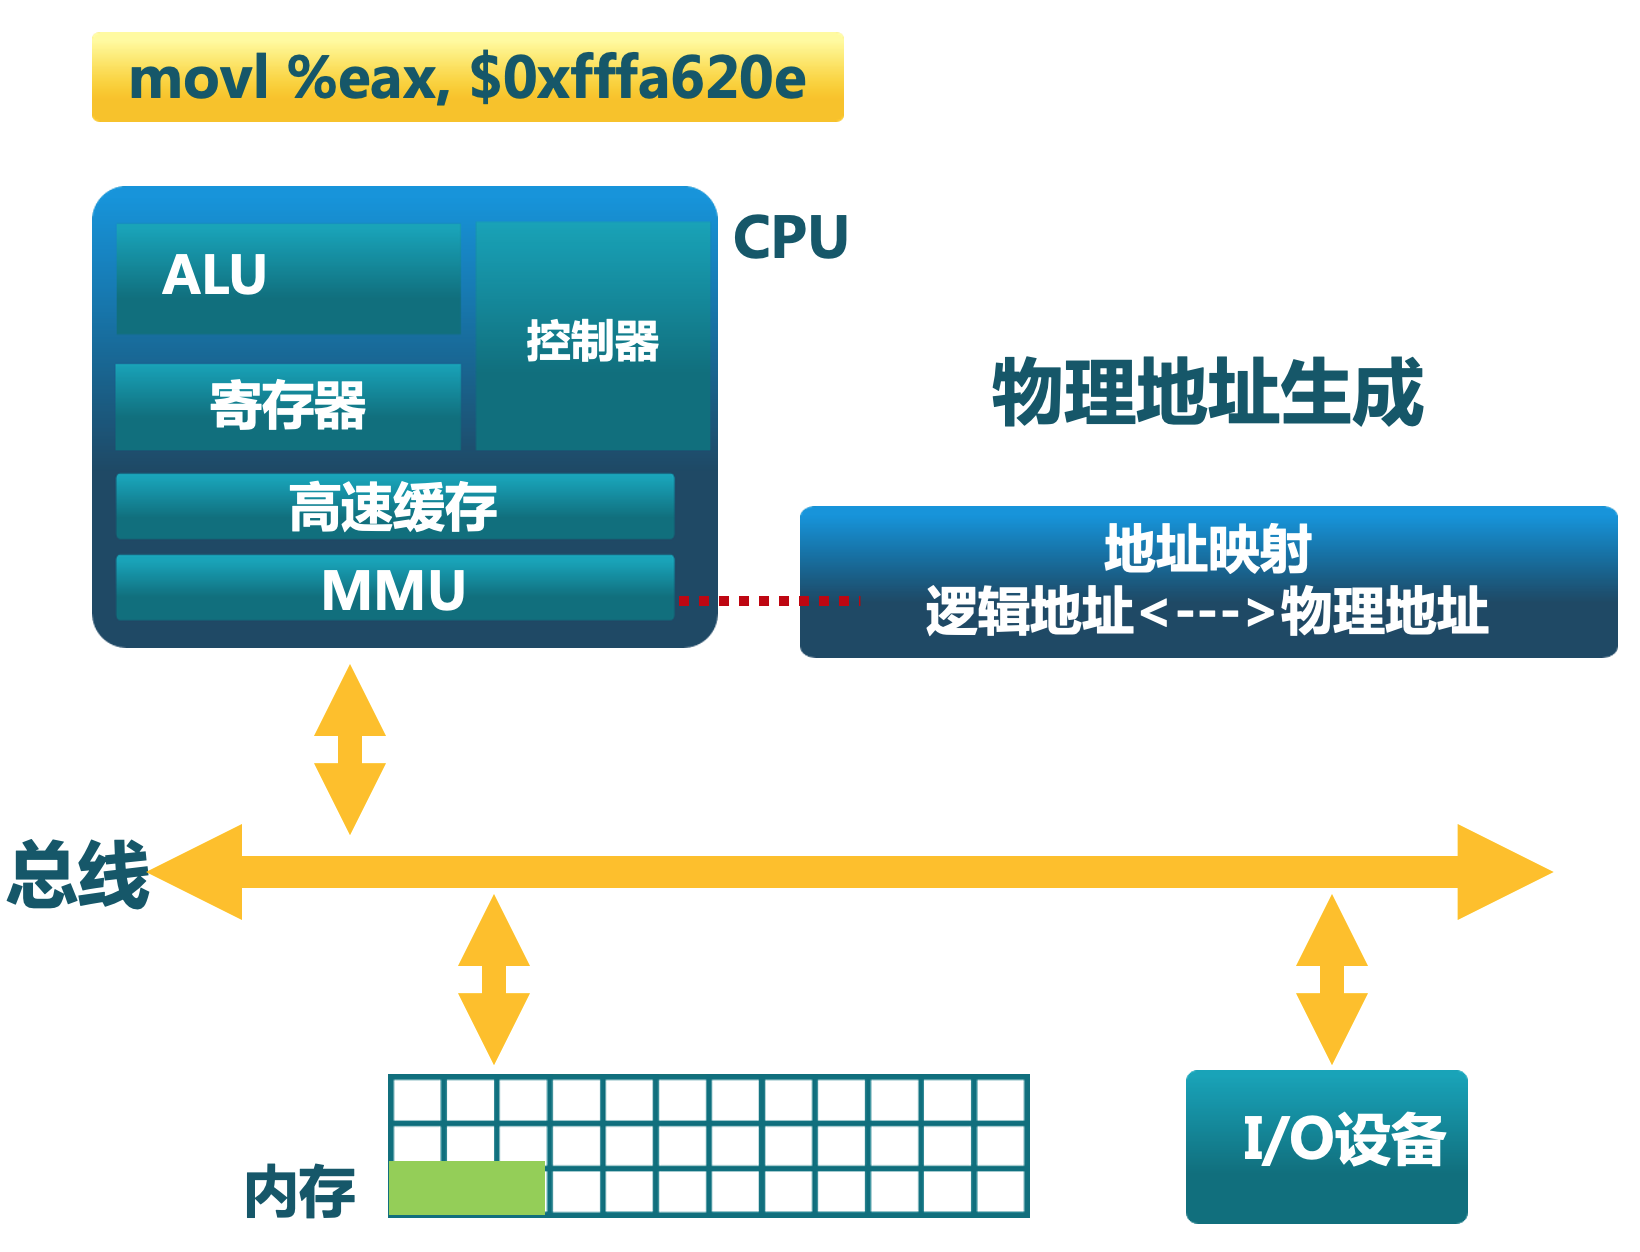
\includegraphics[width=0.7\linewidth]{flow}
		        \caption{xxxx}
		    \end{figure}
	    \end{column}
	    \begin{column}{0.5\textwidth}
			\begin{itemize}
			    \item CPU
			    \begin{itemize}
			        \item ALU:需要逻辑地址的内存内容
			        \item MMU:进行逻辑地址和物理地址的转换
			        \item CPU控制逻辑:给总线发送物理地址请求
			    \end{itemize}
			    \item 内存
			    \begin{itemize}
			        \item 发送物理地址的内容给CPU
			        \item 或接收CPU数据到物理地址
			    \end{itemize}
			    \item 操作系统
			    \begin{itemize}
			        \item 建立逻辑地址LA和物理地址PA的映射
			    \end{itemize}
			\end{itemize}
	    \end{column}
	\end{columns}
    
\end{frame}
%------------------------------------------------
\subsection{地址检查} % A subsection can be created just before a set of slides with a common theme to further break down your presentation into chunks
%------------------------------------------------
\begin{frame}[plain,t]
    
    \frametitle{地址检查}
    
    \begin{figure}
        \centering
        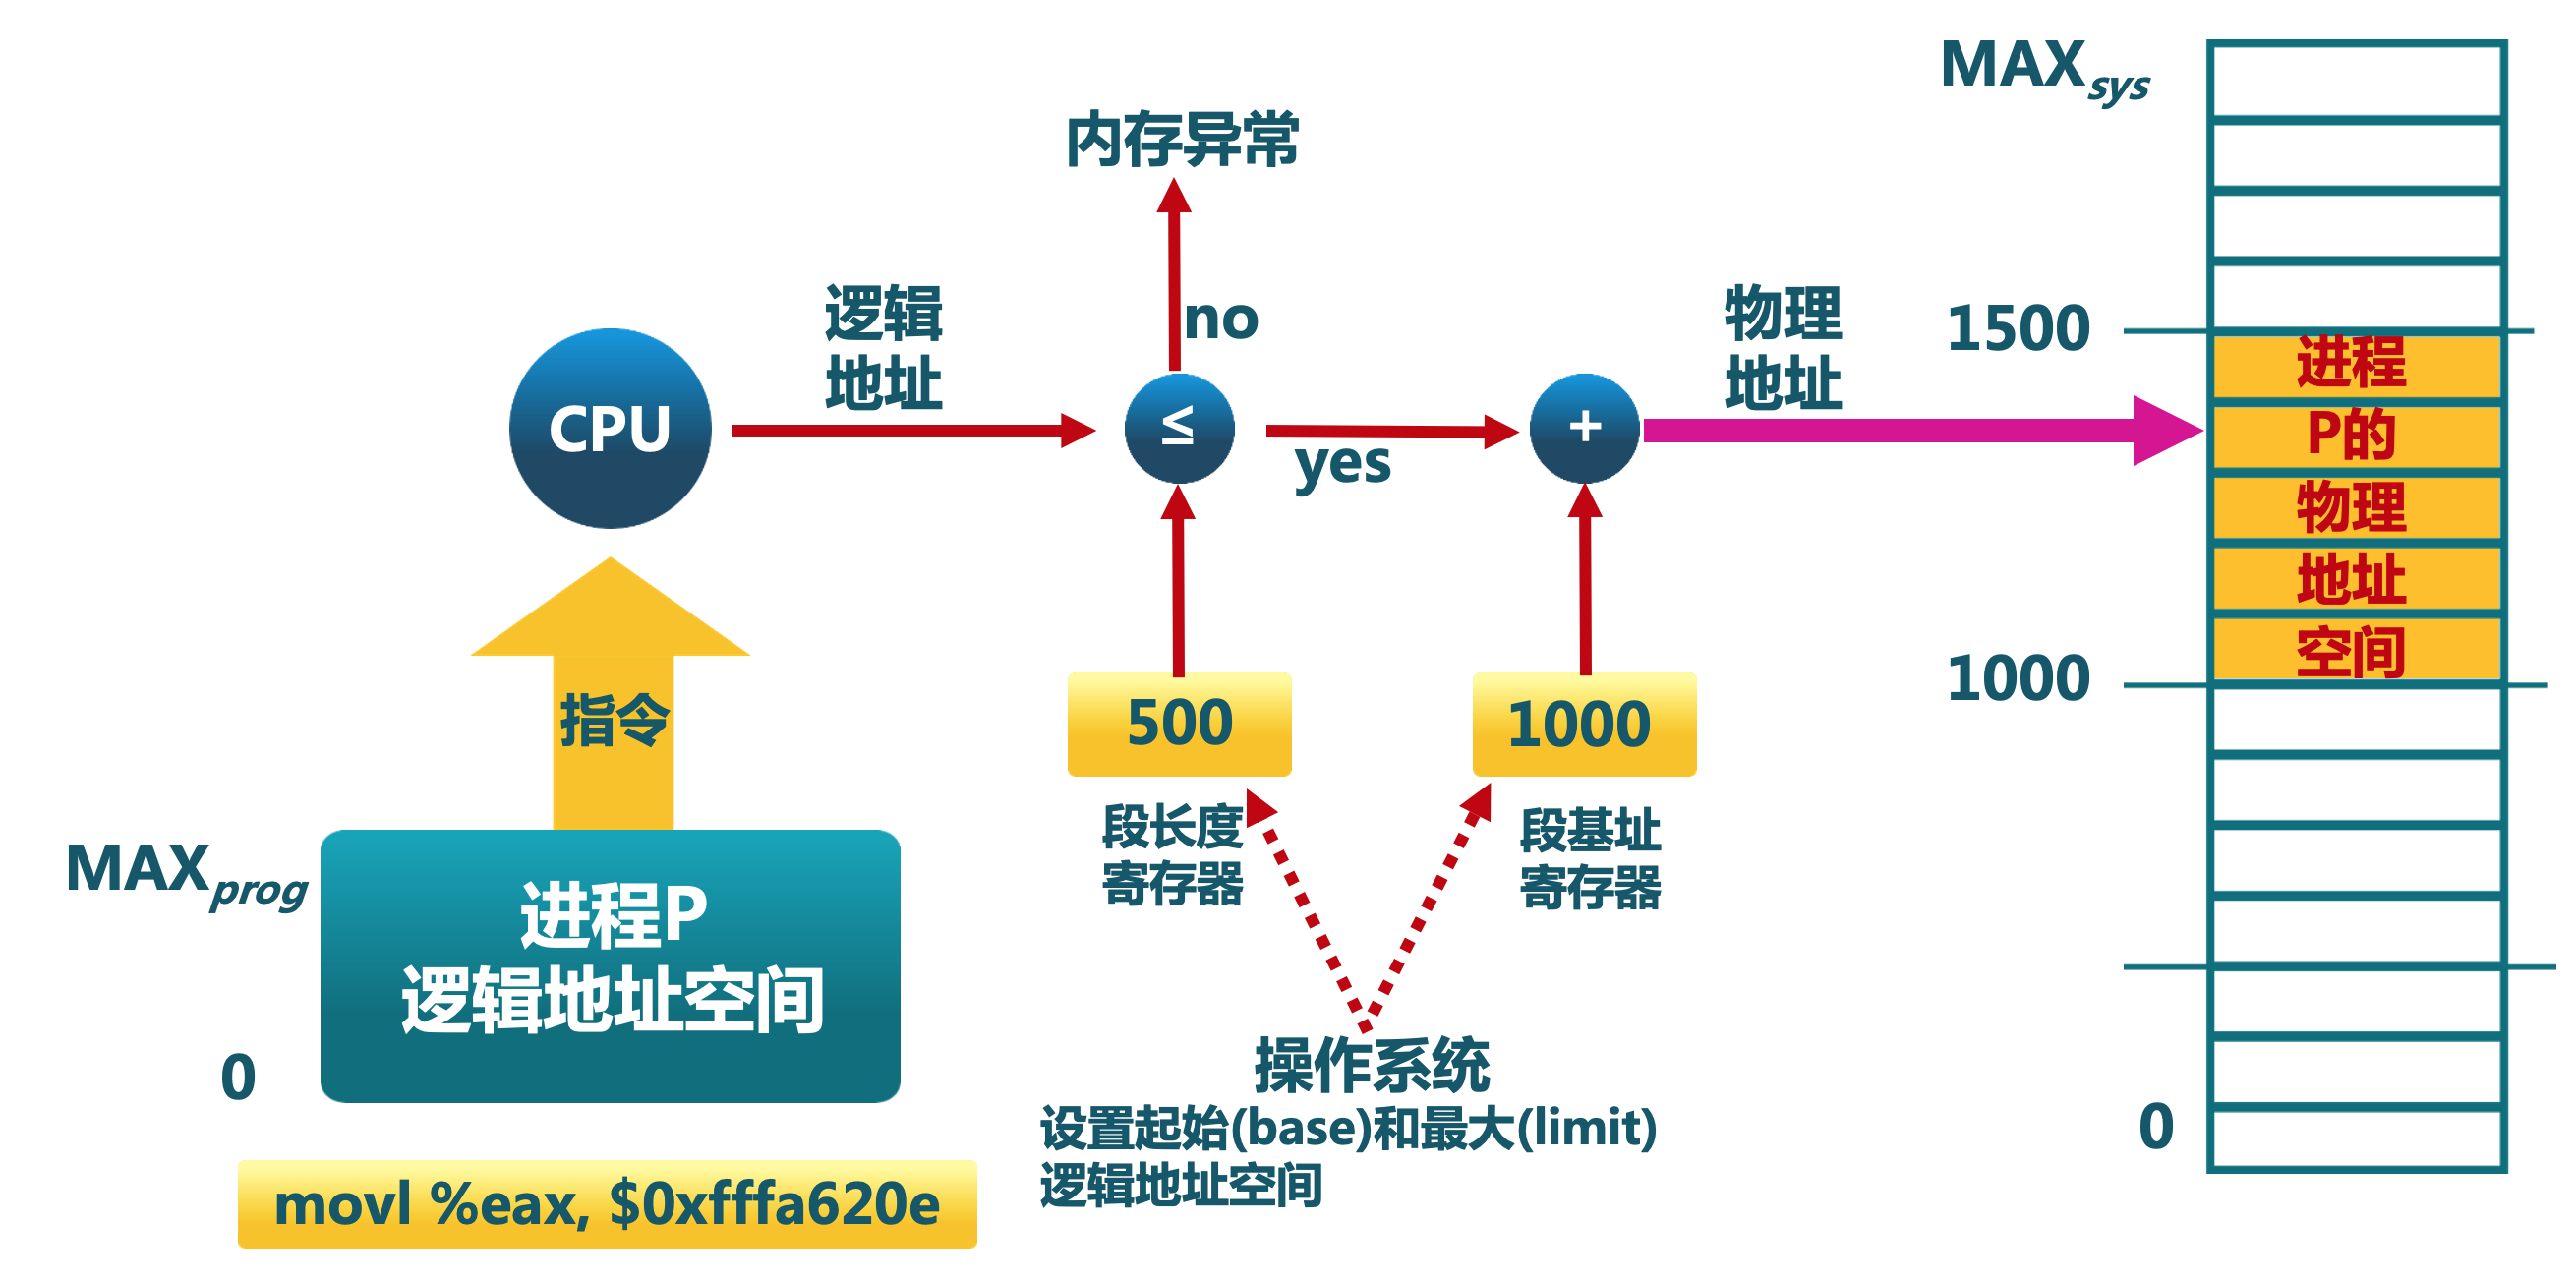
\includegraphics[width=0.7\linewidth]{addr-check}
        \caption{xxxx}
    \end{figure}
    
\end{frame}
%------------------------------------------------
%----------------------------------------------------------------------------------------

\end{document}
